%
% File acl2021.tex
%
%% Based on the style files for EMNLP 2020, which were
%% Based on the style files for ACL 2020, which were
%% Based on the style files for ACL 2018, NAACL 2018/19, which were
%% Based on the style files for ACL-2015, with some improvements
%%  taken from the NAACL-2016 style
%% Based on the style files for ACL-2014, which were, in turn,
%% based on ACL-2013, ACL-2012, ACL-2011, ACL-2010, ACL-IJCNLP-2009,
%% EACL-2009, IJCNLP-2008...
%% Based on the style files for EACL 2006 by 
%%e.agirre@ehu.es or Sergi.Balari@uab.es
%% and that of ACL 08 by Joakim Nivre and Noah Smith

\documentclass[11pt,a4paper]{article}
\usepackage{graphicx}

\usepackage[hyperref]{acl2021}
\usepackage{times}
\usepackage{float}
\usepackage{booktabs}
\usepackage{latexsym}
\renewcommand{\UrlFont}{\ttfamily\small}

% This is not strictly necessary, and may be commented out,
% but it will improve the layout of the manuscript,
% and will typically save some space.
\usepackage{microtype}

\aclfinalcopy % Uncomment this line for the final submission
%\def\aclpaperid{***} %  Enter the acl Paper ID here

%\setlength\titlebox{5cm}
% You can expand the titlebox if you need extra space
% to show all the authors. Please do not make the titlebox
% smaller than 5cm (the original size); we will check this
% in the camera-ready version and ask you to change it back.

\newcommand\BibTeX{B\textsc{ib}\TeX}

\title{Homework 1: Word-in-Context disambiguation}

\author{Leonardo Emili \\
  Sapienza University of Rome, Italy \\
  \texttt{emili.1802989@studenti.uniroma1.it}}

\date{}

\begin{document}
\maketitle
\begin{abstract}
  Word-in-context (WiC) disambiguation is a binary classification task that aims at recognizing whether two target words share the same meaning within two different contexts. Although it may look trivial in its formulation, the task has to deal with a good level of semantics since many words are polysemous in nature: the meaning of a word is heavily influenced by "the company it keeps", Firth (1957). In this work, we present a Bi-LSTM based architecture that leverages sequence encoding to provide a context-aware classification of the input sentences.
\end{abstract}

\section{Introduction}

The homework involved the implementation of a Multi-layer Perceptron (MLP) architecture that makes use of individual word-level information to output the final decision. From this point on, we will refer to it as the \emph{baseline} model. A more sophisticated approach required the use of Recurrent Neural Networks (RNN) to encode context-level information that we expected to boost the overall performances. In the following, we will go through an in-depth analysis of the adopted strategies and the ideas that are rooted in the NLP best practices.

\section{Preprocessing}

For this task, we are provided with an input corpus of the form \emph{sentence\textsubscript{1}}, \emph{sentence\textsubscript{2}}, \emph{target\textsubscript{1}}, \emph{target\textsubscript{2}}, and \emph{label}. In particular, for each sentence pair, we have a gold annotation in the form of a binary label that indicates whether the two target words share the same meaning or not, as well as their position in the original sentence. Moreover, we are provided with additional information for the target words, such as their lemma forms and the respective Part-of-speech (POS) tag. As the first step of the text processing pipeline, we apply tokenization to identify the words that compose our sentences and extract their lemma form. Next, we apply a function over the tokenized data responsible for transforming raw text into values that our models can easily handle. Traditionally in NLP, we distinguish two well-known concepts involved in this process: the \emph{vectorizer function} that applies the previously mentioned transformation, and the \emph{vocabulary} which is represented by the set of unique words in the training set.

\subsection{Vocabulary}

Starting from the training data, we extracted the set of unique tokens (i.e. the \emph{word types}) and assigned to each of them a unique index for the encoding step. It is common practice to define two additional tokens, namely the $<$UNK$>$ and $<$PAD$>$ tokens, and add them to the vocabulary. It is important to note that while the former is one of the available techniques to model \emph{Out-Of-Vocabulary} (OOV) words, the latter is particularly useful when training with mini-batches of variable-length sequences.
Furthermore, we built our vocabulary filtering out those rare words that only appeared once in the training corpus, also known as \emph{Hapax Legomena}.

\section{Pretrained word embeddings}

In this project, we relied on pre-trained 300-dimensional word embeddings that have been trained using Word2Vec \cite{mikolov2013efficient} on the Google News dataset. Furthermore, we also experimented using GloVe embeddings \cite{pennington2014glove} and draw a comparative analysis of the two approaches. The choice of using pre-trained embeddings was a fundamental one. In fact, it let us save a considerable amount of training time and also provided us with high-quality word embeddings.

\section{Models architecture}

In this section, we present both the architectures we implemented, with a particular focus on the recurrent nature of the second approach. Let's start with the simplest one: it is a Multi-Layer Perceptron (MLP) and leverages word embeddings information to classify an input sentence pair. Here we employ a basic aggregation strategy that considers the arithmetic mean over the sequences and passes them through a collection of fully connected layers with ReLu and sigmoid as activation functions. The second approach is somehow similar to the former but also includes an LSTM layer. Furthermore, it makes use of dropout as a strong regularizer as described in \cite{hinton2012improving}. It is worth noting that even though the very same aggregation strategy is used after the LSTM layer, its simplicity has been shown to be effective and provided us with good results, as we will see in the next section. Please refer to Figure 4 for a complete overview of the final architecture.

\subsection{Bidirectional LSTM}

For the sake of this project, we implemented a Bidirectional Long Short-Term Memory (BiLSTM) that is an evolution of the simpler LSTM model. The basic intuition behind recurrent neural networks (RNN) is that we can leverage the sequential nature of an input sequence and extrapolate some context-aware representation from the input words. More in detail, we provide input sentences to the network in a time step fashion, where at each time step some input $x_i$ of the original sentence $x$ is fed to the network. In this way, the latent representation of feature $x_i$, a word embedding in our case, will also take into account the history $h_i=(x_1, x_2, ..., x_{i-1})$. It confirms our intuition that the meaning of a word is encoded by its neighboring words, hence we expect to get a better understanding of the input sentence compared to simpler models (e.g. MLP). Our choice of using an LSTM architecture over vanilla RNNs comes from the fact that they better handle the vanishing gradient problem. For the sake of this report, we will not delve too much into detail. However, it is important to note that their gated architecture enables them to learn short-term dependencies while also retaining part of long-term dependencies. Furthermore, using a BiLSTM, we get a better understanding of the context of a word since we are observing its neighboring tokens in both directions.

\section{Results}

In this section, we draw a quantitative evaluation of the performances of the proposed models on actual test data. It is worth noting that we retained a few samples from the train set to test the model performances on unseen data and observed similar results. As mentioned in previous sections, we expected the recurrent model to outperform the simpler multi-layer perceptron. After careful fine-tuning operations, the baseline model was able to score 63.57\% of F1. No further data preprocessing, such as removing rare words from the vocabulary or putting the dataset lowercase, helped in this case. Whether instead, we analyze the recurrent model, we observe a notable performance gain applying such techniques. The best overall model configuration, described in Table 3, let us reach a 69.14\% of F1 score. Here, we applied a threshold mechanism to filter out words with frequency one in the training set, as explained in Section 2.1, which showed to be effective in this case. In Figure 3, we can better visualize its capabilities and observe that the false negatives are fewer than false positives. From Table 2, we can observe the results of different experiments using pre-trained embeddings from Word2Vec and GloVe. GloVe embeddings proved to be less effective in this case, and we believe it is partially due to the vocabulary size. In particular, using the latter solution, we discovered that some words were not available with GloVe embeddings, potentially finding a higher number of OOV words at test time. As an additional experiment (*), we concatenated Word2Vec and GloVe embeddings together. In this experiment (**), we also considered the case where one of the two embeddings was missing and concatenated the available one to itself. Both of them were able to outperform any of the above MLP-based solutions but did not improve the results further. We can observe from Figures 1 and 2 that the model did not suffer from overfitting.

\section{Conclusions}

In this project, we explored different solutions and showed the effectiveness of recurrent neural networks when dealing with sequential data. As a further exploration step, it would be interesting to leverage more sophisticated approaches such as contextualized embeddings as a way of incorporating semantics into the task. Moreover, adding more features such as POS embeddings or char embeddings could improve the performance further.

\bibliographystyle{acl_natbib}
\bibliography{anthology,acl2021}

\begin{figure}[H]
  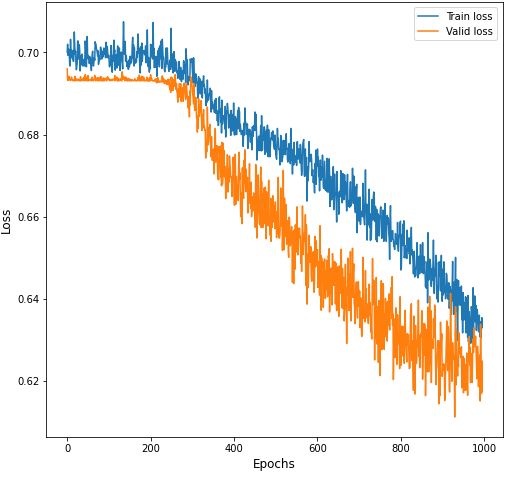
\includegraphics[width=8.2cm,keepaspectratio]{images/loss.png}
  \caption{Training/validation loss of the best overall model over the training epochs.}\label{fig:lstm_loss}
\end{figure}

\begin{figure}[H]
  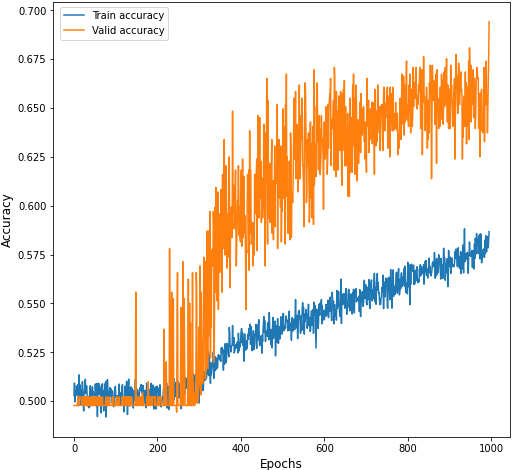
\includegraphics[width=8.2cm,keepaspectratio]{images/accuracy.png}
  \caption{Training/validation accuracy of the best overall model over the training epochs.}\label{fig:lstm_accuracy}
\end{figure}

\begin{table}[H]
  \centering
  \begin{tabular}{lr} \toprule
  \textbf{Model} & \textbf{F1 (\%)} \\ \midrule
  MLP & 62.85 \\
  + lemmatization & \textbf{63.57} \\
  + rare words removal & 61.17 \\
  + lowercase & 61.28 \\ \midrule
  BiLSTM  & 67.6 \\
  + lemmatization & 68.3 \\
  + rare words removal & \textbf{69.14} \\
  + lowercase & 67.73 \\
  \bottomrule
  \end{tabular}
  \caption{\label{word2vec_models} Performance comparison of the two architectures under different configuration scenarios using pre-trained embeddings from Word2Vec. }
\end{table}

\begin{table}[H]
  \centering
  \begin{tabular}{lr} \toprule
  \textbf{Embedding} & \textbf{F1 (\%)} \\ \midrule
  Word2Vec  & \textbf{69.14} \\
  300d GloVe & 64.77 \\
  Word2Vec $\oplus$ 300d GloVe \footnotesize{\textsuperscript{(*)}} & 66.05 \\
  Word2Vec $\oplus$ 300d GloVe \footnotesize{\textsuperscript{(**)}} & 66.18 \\
  \bottomrule
  \end{tabular}
  \caption{\label{embedding_models} Performance comparison of the best performing models using different types of word embeddings. }
\end{table}

\begin{table}[H]
  \centering
  \begin{tabular}{lr} \toprule
  \textbf{Hyperparameter} & \textbf{Value} \\ \midrule
  optimizer  & SGD \\
  loss function  & BCE \\
  learning rate  & 0.06 \\
  momentum  & 0.92 \\
  dropout & 0.65 \\
  \bottomrule
  \end{tabular}
  \caption{\label{lstm_hparams} List of hyperparameters of the best performing BiLSTM model after the hyperparameter tuning phase. }
\end{table}

\begin{figure}[H]
  \centering
  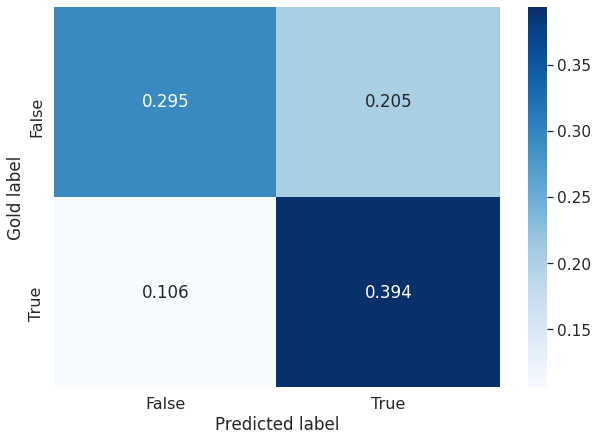
\includegraphics[width=8.45cm,keepaspectratio]{images/confusion_matrix.png}
  \caption{Normalized confusion matrix for the best performing LSTM model using Word2Vec embeddings.}\label{fig:cf}
\end{figure}

\begin{figure}[H]
  \centering
  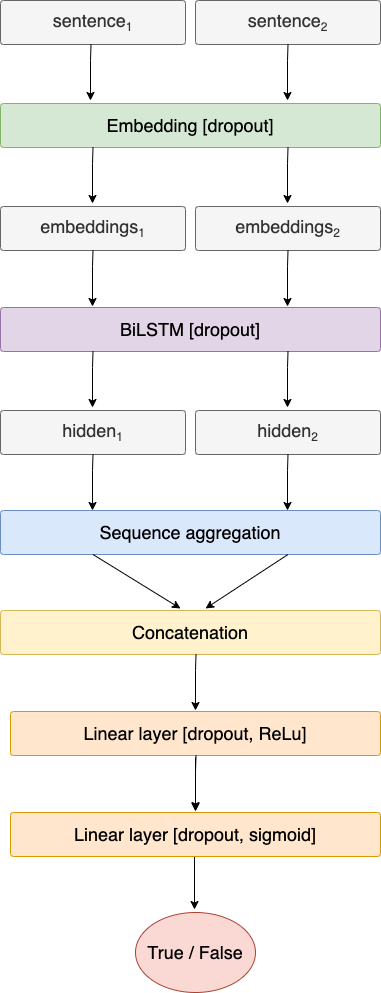
\includegraphics[width=7cm,keepaspectratio]{images/LSTM_architecture.png}
  \caption{Overview of the BiLSTM model architecture that takes a sentence pair as input, encodes them through an embedding layer and aggregates the BiLSTM encodings over the sequence lengths. Ultimately, the two representations are concatenated and fed to two fully connected layers to predict the final decision.}\label{fig:architecture}
\end{figure}

\end{document}
